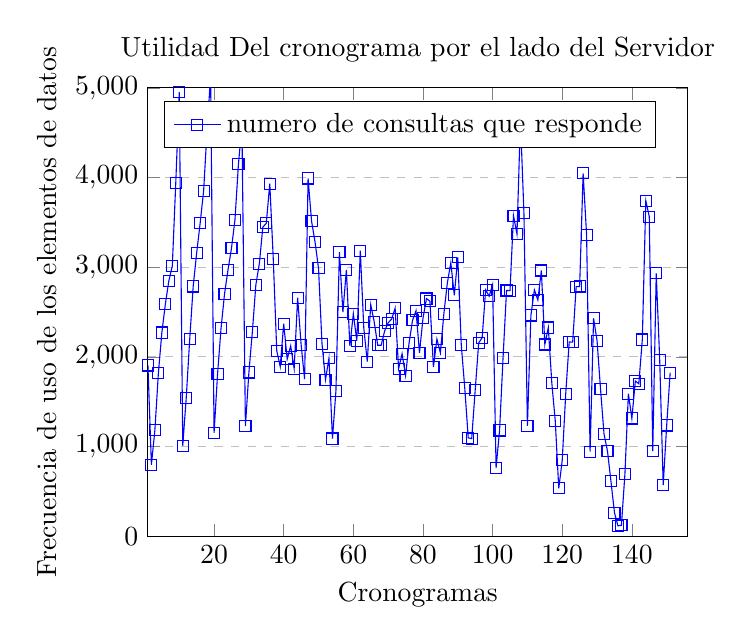
\begin{tikzpicture}
\begin{axis}[
    title={Utilidad Del cronograma por el lado del Servidor},
    xlabel={Cronogramas},
    ylabel={Frecuencia de uso de los elementos de datos},
    xmin=1, xmax=156,
    ymin=0, ymax=5000,
    xtick={},
    ytick={},
    legend pos=north west,
    ymajorgrids=true,
    grid style=dashed,
]

\addplot[
    color=blue,
    mark=square,
    ]
    coordinates {
%UTILIDAD TOTAL
(1,1904)
(2,797)
(3,1183)
(4,1816)
(5,2271)
(6,2586)
(7,2847)
(8,3012)
(9,3943)
(10,4951)
(11,1009)
(12,1541)
(13,2195)
(14,2785)
(15,3159)
(16,3491)
(17,3853)
(18,4533)
(19,5127)
(20,1152)
(21,1808)
(22,2318)
(23,2701)
(24,2970)
(25,3212)
(26,3528)
(27,4149)
(28,4577)
(29,1228)
(30,1826)
(31,2281)
(32,2804)
(33,3038)
(34,3446)
(35,3491)
(36,3932)
(37,3094)
(38,2068)
(39,1891)
(40,2371)
(41,1975)
(42,2122)
(43,1869)
(44,2660)
(45,2136)
(46,1751)
(47,3990)
(48,3514)
(49,3280)
(50,2988)
(51,2146)
(52,1746)
(53,1986)
(54,1089)
(55,1621)
(56,3169)
(57,2498)
(58,2969)
(59,2122)
(60,2481)
(61,2179)
(62,3184)
(63,2321)
(64,1947)
(65,2582)
(66,2388)
(67,2129)
(68,2130)
(69,2290)
(70,2381)
(71,2421)
(72,2543)
(73,1868)
(74,2035)
(75,1791)
(76,2152)
(77,2407)
(78,2514)
(79,2044)
(80,2430)
(81,2650)
(82,2620)
(83,1887)
(84,2198)
(85,2045)
(86,2481)
(87,2824)
(88,3050)
(89,2687)
(90,3110)
(91,2133)
(92,1654)
(93,1097)
(94,1088)
(95,1629)
(96,2155)
(97,2213)
(98,2746)
(99,2676)
(100,2805)
(101,762)
(102,1179)
(103,1988)
(104,2740)
(105,2739)
(106,3575)
(107,3370)
(108,4643)
(109,3605)
(110,1230)
(111,2462)
(112,2747)
(113,2634)
(114,2963)
(115,2138)
(116,2327)
(117,1713)
(118,1285)
(119,533)
(120,847)
(121,1588)
(122,2166)
(123,2164)
(124,2783)
(125,2785)
(126,4047)
(127,3359)
(128,942)
(129,2430)
(130,2181)
(131,1640)
(132,1140)
(133,947)
(134,611)
(135,263)
(136,115)
(137,121)
(138,691)
(139,1590)
(140,1313)
(141,1730)
(142,1700)
(143,2193)
(144,3742)
(145,3564)
(146,948)
(147,2931)
(148,1961)
(149,571)
(150,1235)
(151,1824)
    };
    \legend{numero de consultas que responde}

\end{axis}
\end{tikzpicture}

